\subsection{Photon-Counting in Film Photography}

The principal notions of the single-bit imaging sensors can be traced back to analog photography and demonstrate behaviors reminiscent to ones of the silver halide emulsion, a common component in the photographic film. 

Akin to its digital counterpart, the photographic film is subjected to the photoelectric effect; in film, this is represented by the photographic emulsion coated on the transparent sheet of plastic. Such emulsion consists of microscopic crystals, or grains, of silver halides embedded in protective colloid like gelatin \cite{Carroll1980}, with the commonly considered compounds being silver bromide \textit{AgBr}, silver chloride \textit{AgCl}, silver iodide \textit{AgI}, or some mixture thereof \cite{Schroeder1981}.
%ionenbindung löst photographischen primärprozess: elektron durch quantenenergie abgespalten; wirkung des primproz ist srtreng proportional zu der quantenzahl!
\begin{figure}[h]
  \centering
  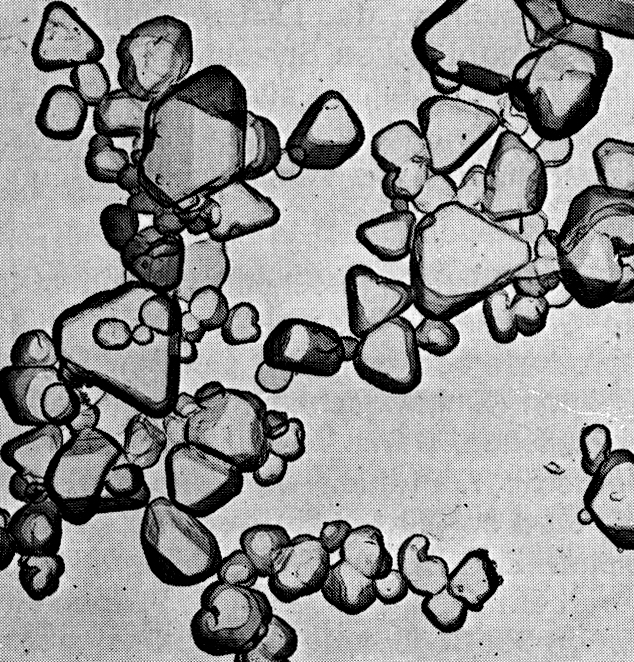
\includegraphics[width=0.5\linewidth]{imgs/film/silver.jpg}
  \caption{Electron microscopic structure of undeveloped silver bromide crystals, via \cite{AgfaABC}.}
  \label{fig:silverbromide}
  \Description{Small blackish crystals of silver on gray background}
\end{figure}

The process starts upon exposure of the film to the light. Film grains absorb the incoming radiation in form of the incident photons and dissociate into a group of free silver ions. 

Once exposed to development agent, the silver ions in the film are reduced to metallic silver, rendering the exposed regions of the film sheet opaque black. The unaltered halides are later dissolved out in a chemical bath, so that the corresponding spots are transparent. Each crystal can either be struck by a photon or not, and so the film exhibits a binary response. 

%chance of absorprtion of a photon by a grain; grain must absorb r quanta in order to be developable. when r = 1, equation is reduced to 1-e ^ (-q); the shape of the characteristic curve depends on photon distribution
The exposed grains are spread randomly, fluctuate in size and differ in absorption rate -- there is no uniformity regarding the required absorbed quanta as the particles arrive randomly. However, with the irradiance of the image areas varying, so does the stochastic photon distribution and therefore the concentration of silver particles per film area. 

Fine granular structures are not perceivable by the human eye and are registered as continuous tone of gray \cite{Feng_Yang_2012} instead, matching the overall area density to the original light intensity information; the mean number of absorbed quanta per grain is given by the Poisson equation. % (optical density)

%For conventional sensors some of this non-linear response can be encoded in the postprocessing of the linear-response image. Nevertheless, the non-linear response of film has been hard to match even in HDR solid-state image sensors without introducing artifacts due to motion, threshold voltage fixed- pattern variation, and other circuit design issues

\begin{figure}[h]
  \centering
  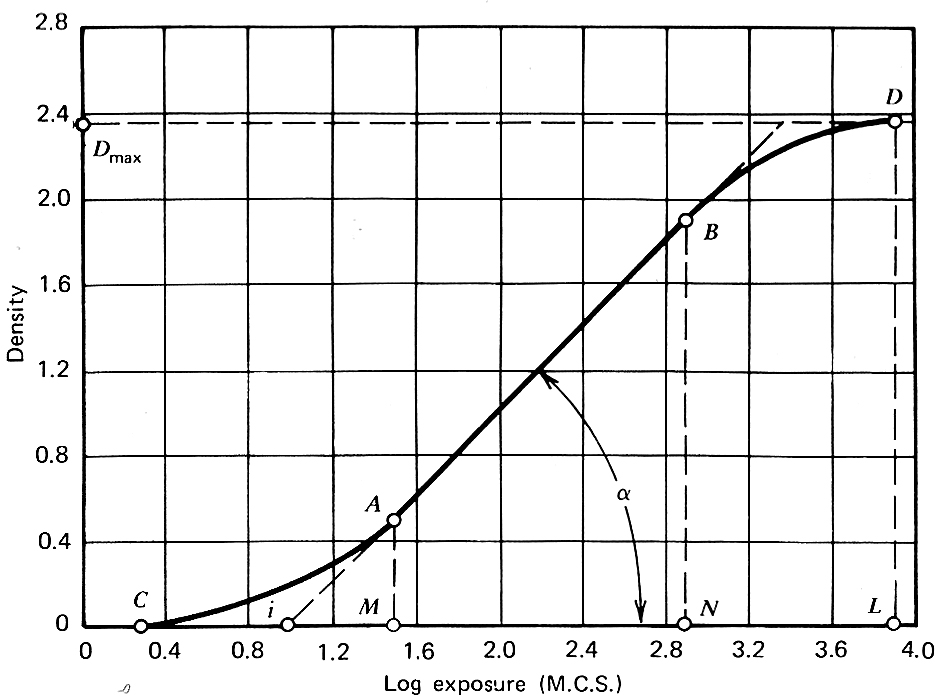
\includegraphics[width=\linewidth]{imgs/film/filmcurve.jpg}
  \caption{Exemplary characteristic curve of the film emulsion, via \cite{Saleh1991}.}
  \label{fig:filmcurve}
  \Description{S-shaped curve relates the optical density to the logarithmic exposure. There are two latitudes on both ends of the curve.}
\end{figure}
The photographic properties of the film emulsion are typically described through the ratio of the luminance transmitted in the medium to the luminance of the observed scene. The optical density is modelled as a function of logarithmic exposure and was first derived in \cite{HurterDriffield}. As seen in Figure \ref{fig:filmcurve}, this relationship has a non-linear behavior. 

The D - log H curve (also referred to as \textit{ characteristic curve}) can be split into three intervals based on the curvature of the response. For sufficiently small or large values of logH, the function is asymptotic and results in under- or overexposure (the toe and shoulder portions of the curve, respectively~\cite{Hunt2005}); in the middle interval, the slope is constant, and the relationship between the luminance and the photographic density is linear. %Under sparse exposures and overexposures, this means better tolerance for highlights
In general, the S-shape of the curve is determined by the underlying randomness of photon arrivals. (This is different in conventional CIS sensors.)

In film, the grains may fluctuate in size, ranging from 0.048 to 1.71 $\mu$m depending on the application; on average, one grain of the developed emulsion corresponds to ca. 3-4 electrons~\cite{Carroll1980, FossumSiMulQIS}. Feature sizes of QIS are similar in their capacitance; the jots in the single-carrier implementation of QIS are meant to store around 3 carriers as well. Thus, both digital sensors QIS and analog film deliver quantized, spatially discrete values obtained off similar area sizes. So, the behavior in binary imaging sensors is, too, dominated by the photon distribution. Resulting characteristic curve is shaped comparably, demonstrating slightly larger overexposure latitude~\cite{FossumSiMulQIS}.

\begin{figure}[h]
  \centering
  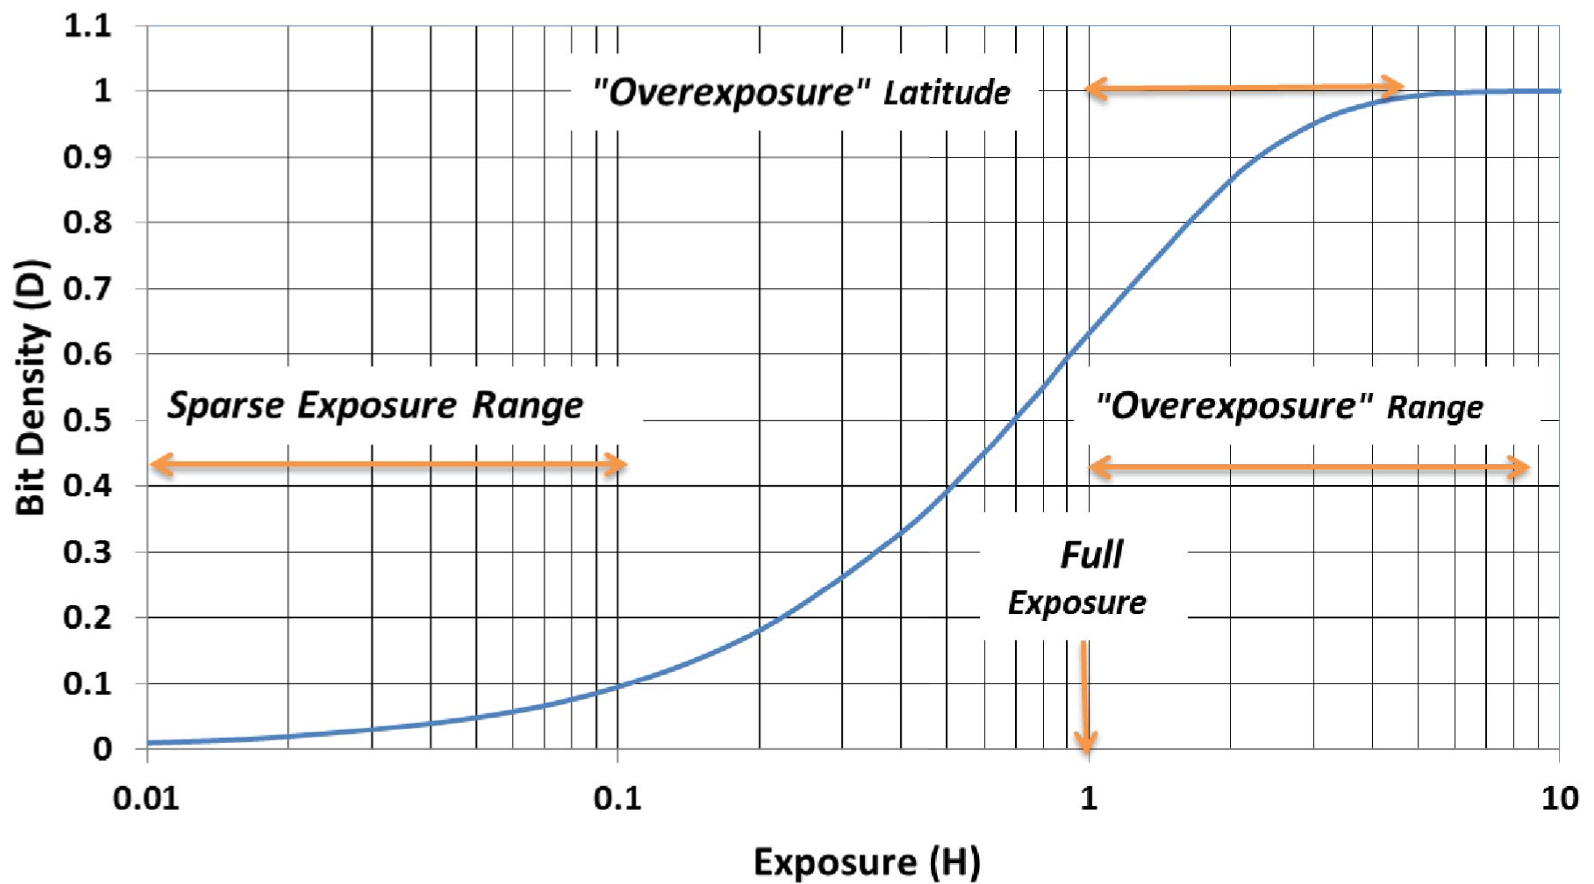
\includegraphics[width=\linewidth]{imgs/film/qiscurve.png}
  \caption{Characteristic curve of the quanta imaging sensor, via \cite{fossum2016quanta}.}
  \label{fig:qiscurve}
  \Description{Shown is the response of the QIS with the S-shaped curve relating the bit density to the exposure.}
\end{figure}

